% --- [ Control Flow Recovery Results ] ----------------------------------------

\subsection{Control Flow Recovery Results}
\label{app:control_flow_recovery_results}

% ~~~ [ Coreutils Test Programs ] ~~~~~~~~~~~~~~~~~~~~~~~~~~~~~~~~~~~~~~~~~~~~~~

\subsubsection{Coreutils Test Programs}
\label{app:coreutils_test_programs}

Results of control flow recovery methods for Coreutils test programs.

\begin{figure}[htbp]
	\centering
	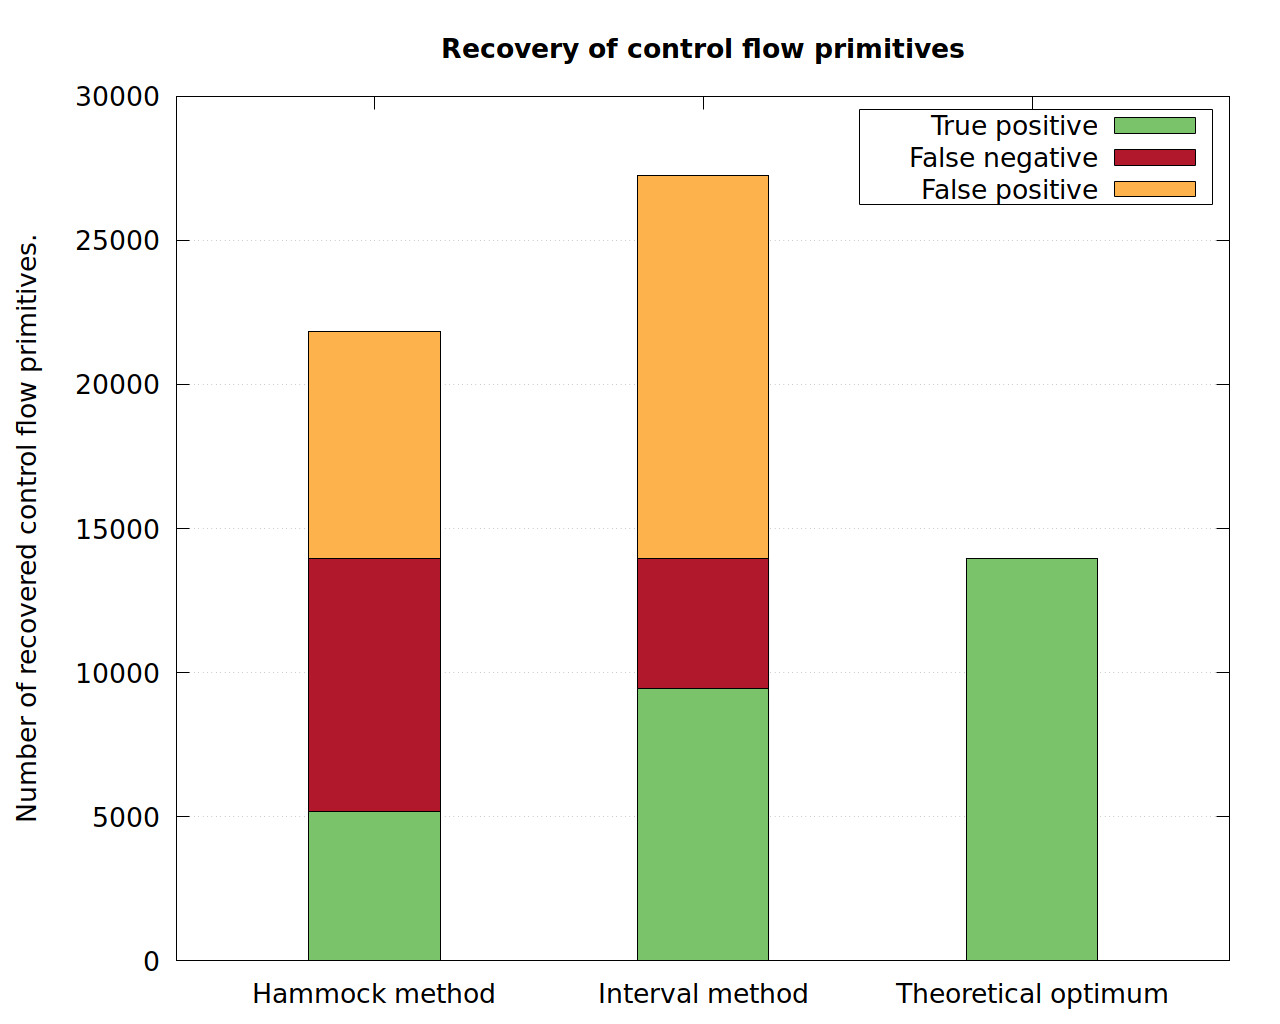
\includegraphics[width=\textwidth]{inc/appendices/test_program_results/coreutils/results_combined.png}
	\caption{Comparison of control flow recovery results for each method, with the combined results of recovering \textit{2-way conditionals}, \textit{n-way conditionals}, \textit{pre-test loops} and \textit{post-test loops}. The data is based on the test programs of Coreutils.}
	\label{fig:coreutils_results_combined}
\end{figure}

\begin{figure}[htbp]
	\centering
	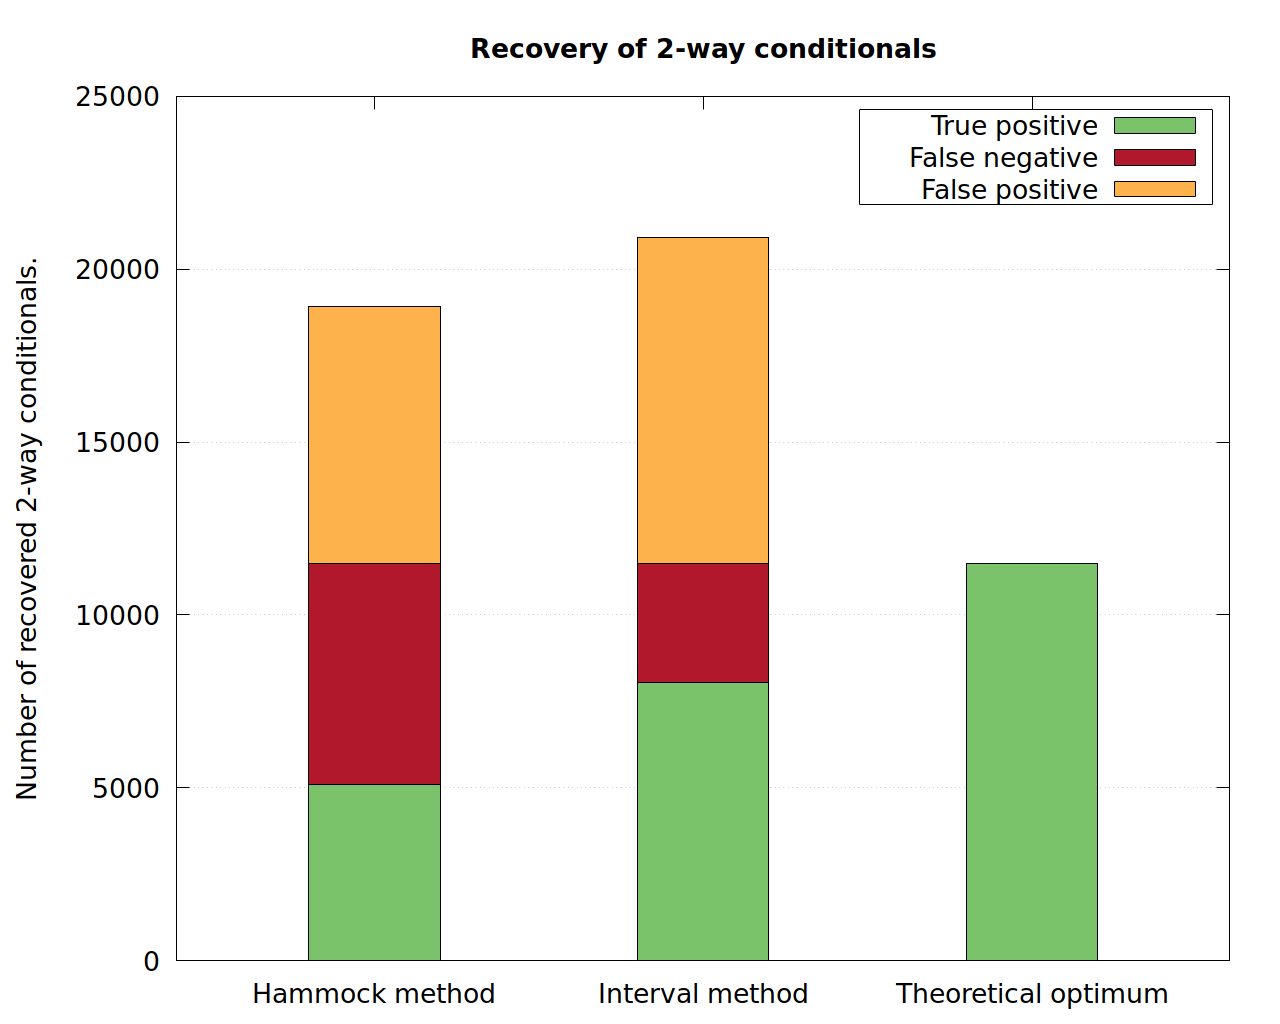
\includegraphics[width=\textwidth]{inc/appendices/test_program_results/coreutils/results_2-way.png}
	\caption{Comparison of control flow recovery results for each method when recovering \textit{2-way conditionals}. The data is based on the test programs of Coreutils.}
	\label{fig:coreutils_results_2way}
\end{figure}

\begin{figure}[htbp]
	\centering
	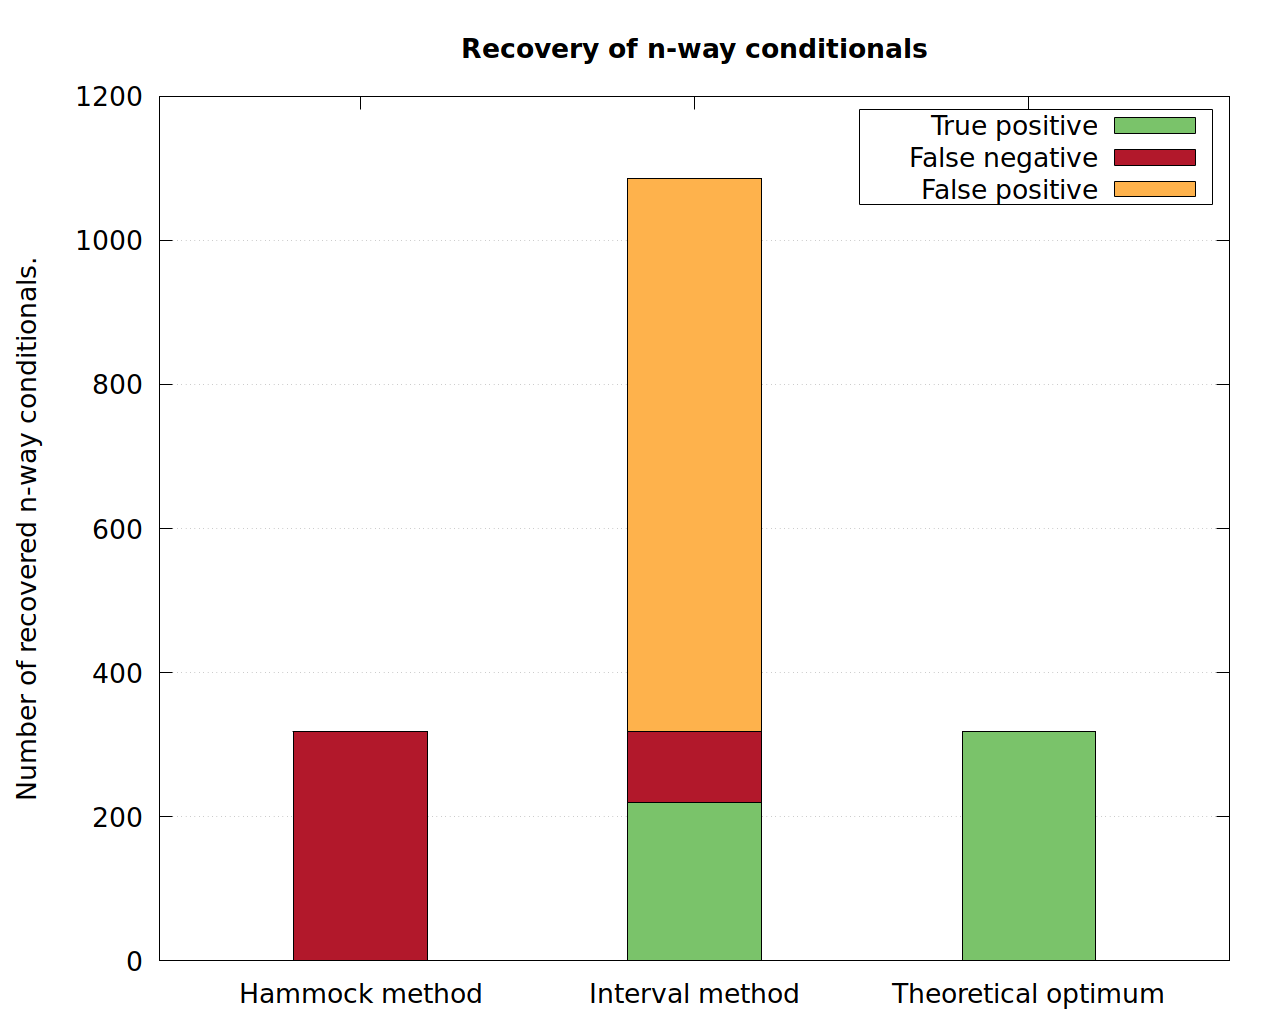
\includegraphics[width=\textwidth]{inc/appendices/test_program_results/coreutils/results_n-way.png}
	\caption{Comparison of control flow recovery results for each method when recovering \textit{n-way conditionals}. The data is based on the test programs of Coreutils.}
	\label{fig:coreutils_results_nway}
\end{figure}

\begin{figure}[htbp]
	\centering
	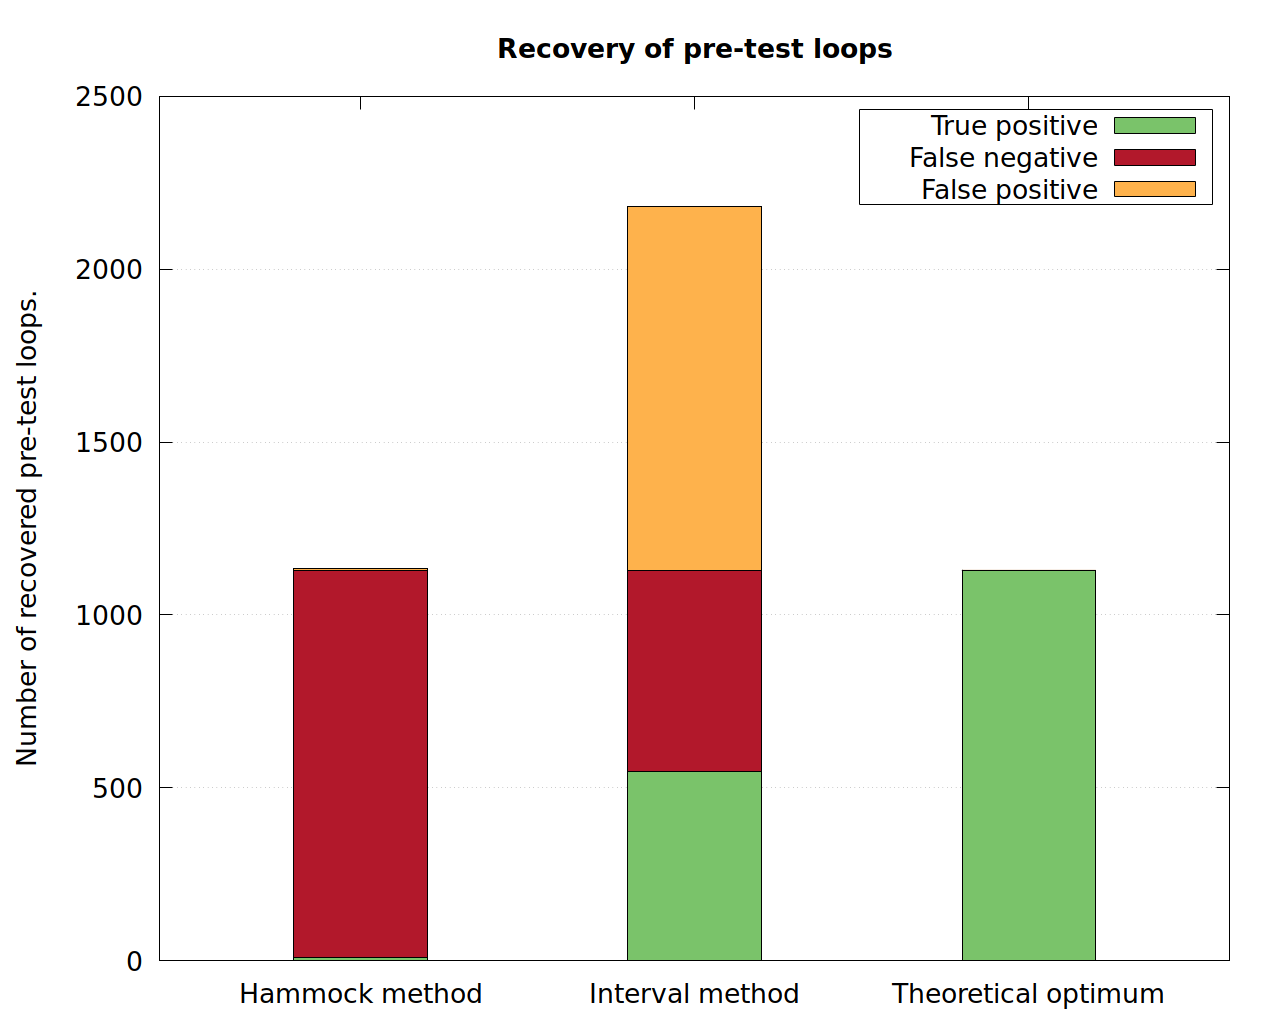
\includegraphics[width=\textwidth]{inc/appendices/test_program_results/coreutils/results_pre_loop.png}
	\caption{Comparison of control flow recovery results for each method when recovering \textit{pre-test loops}. The data is based on the test programs of Coreutils.}
	\label{fig:coreutils_results_pre_loop}
\end{figure}

\begin{figure}[htbp]
	\centering
	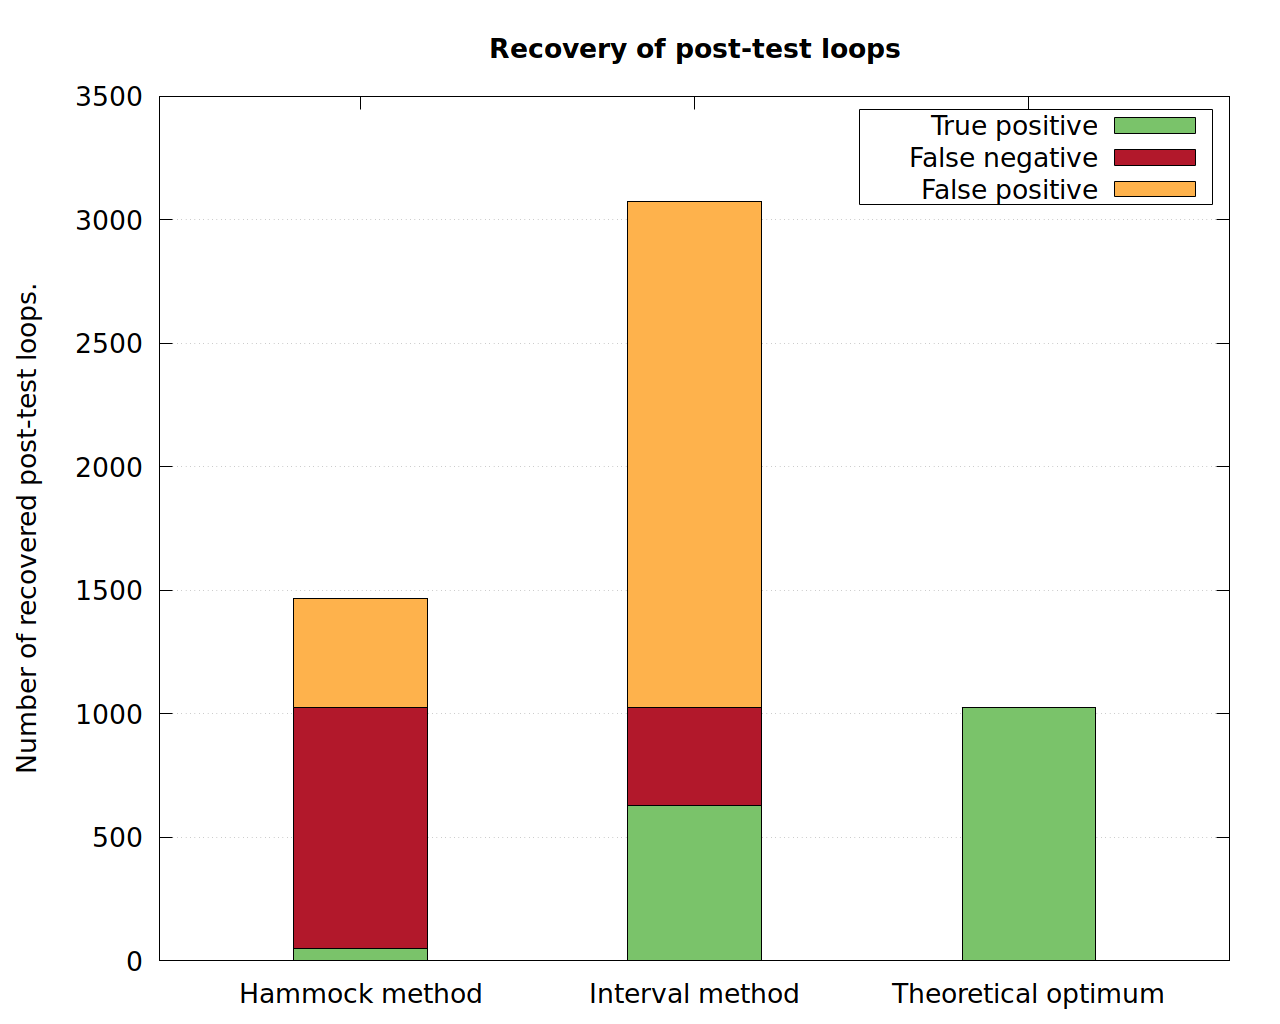
\includegraphics[width=\textwidth]{inc/appendices/test_program_results/coreutils/results_post_loop.png}
	\caption{Comparison of control flow recovery results for each method when recovering \textit{post-test loops}. The data is based on the test programs of Coreutils.}
	\label{fig:coreutils_results_post_loop}
\end{figure}

% ~~~ [ SQLite Test Programs ] ~~~~~~~~~~~~~~~~~~~~~~~~~~~~~~~~~~~~~~~~~~~~~~~~~

\clearpage

\subsubsection{SQLite Test Programs}
\label{app:sqlite_test_programs}

Results of control flow recovery methods for SQLite test programs.

\begin{figure}[htbp]
	\centering
	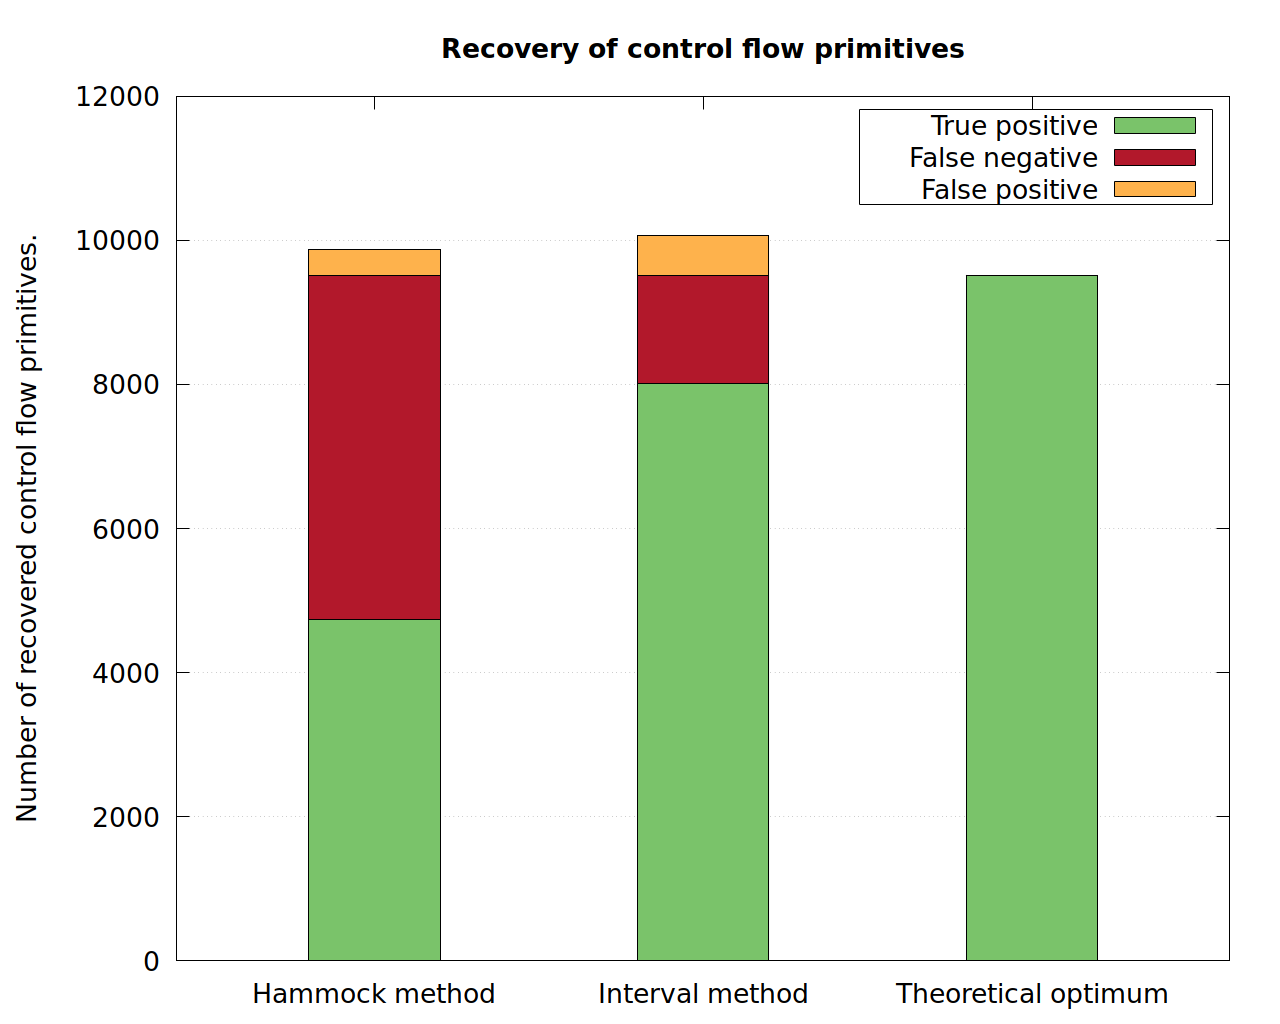
\includegraphics[width=\textwidth]{inc/appendices/test_program_results/sqlite/results_combined.png}
	\caption{Comparison of control flow recovery results for each method, with the combined results of recovering \textit{2-way conditionals}, \textit{n-way conditionals}, \textit{pre-test loops} and \textit{post-test loops}. The data is based on the test programs of SQLite.}
	\label{fig:sqlite_results_combined}
\end{figure}

\begin{figure}[htbp]
	\centering
	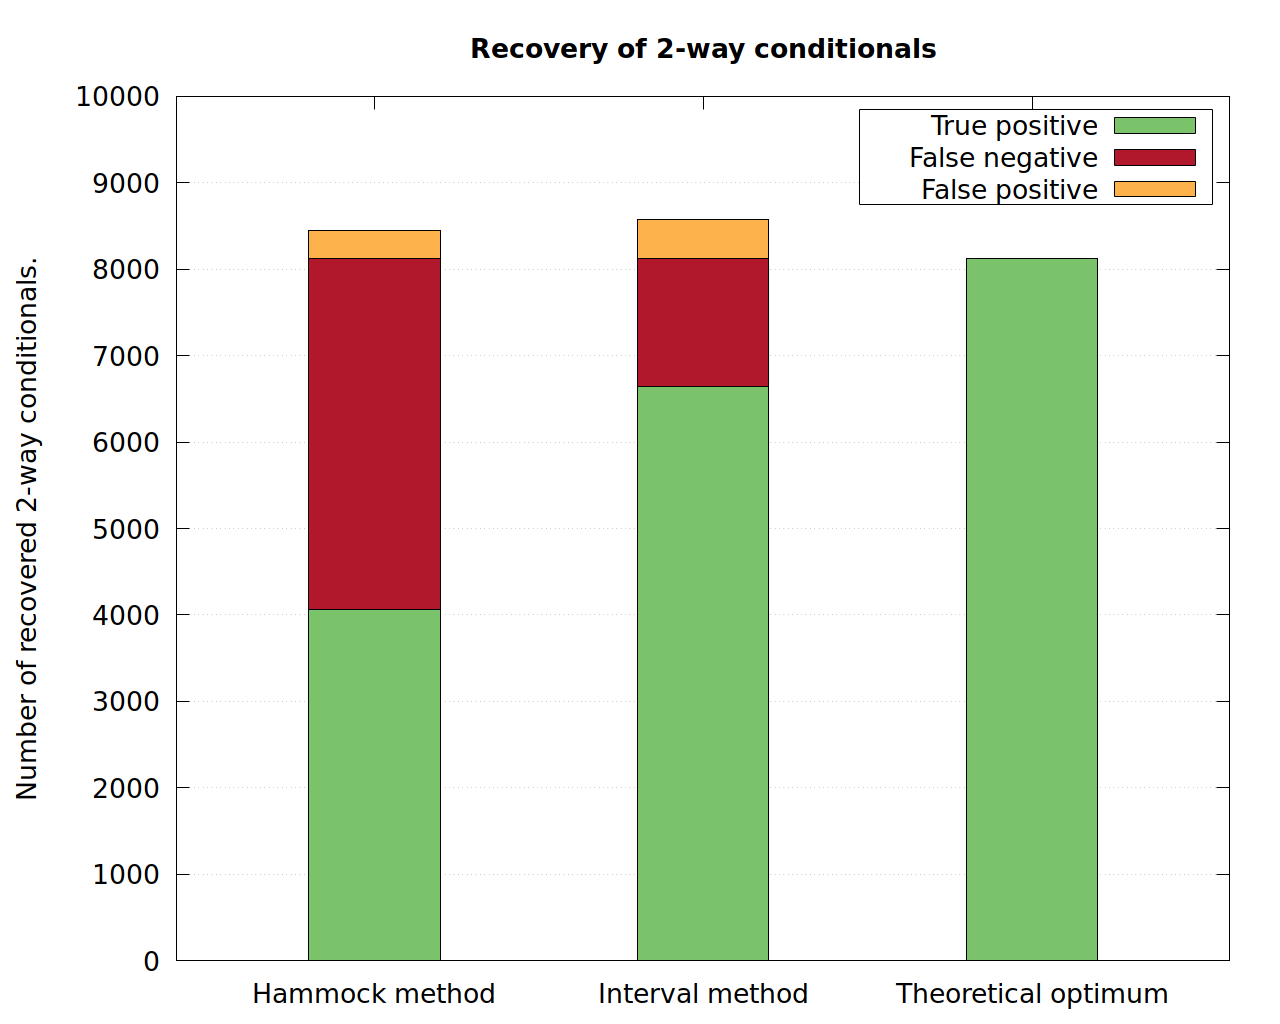
\includegraphics[width=\textwidth]{inc/appendices/test_program_results/sqlite/results_2-way.png}
	\caption{Comparison of control flow recovery results for each method when recovering \textit{2-way conditionals}. The data is based on the test programs of SQLite.}
	\label{fig:sqlite_results_2way}
\end{figure}

\begin{figure}[htbp]
	\centering
	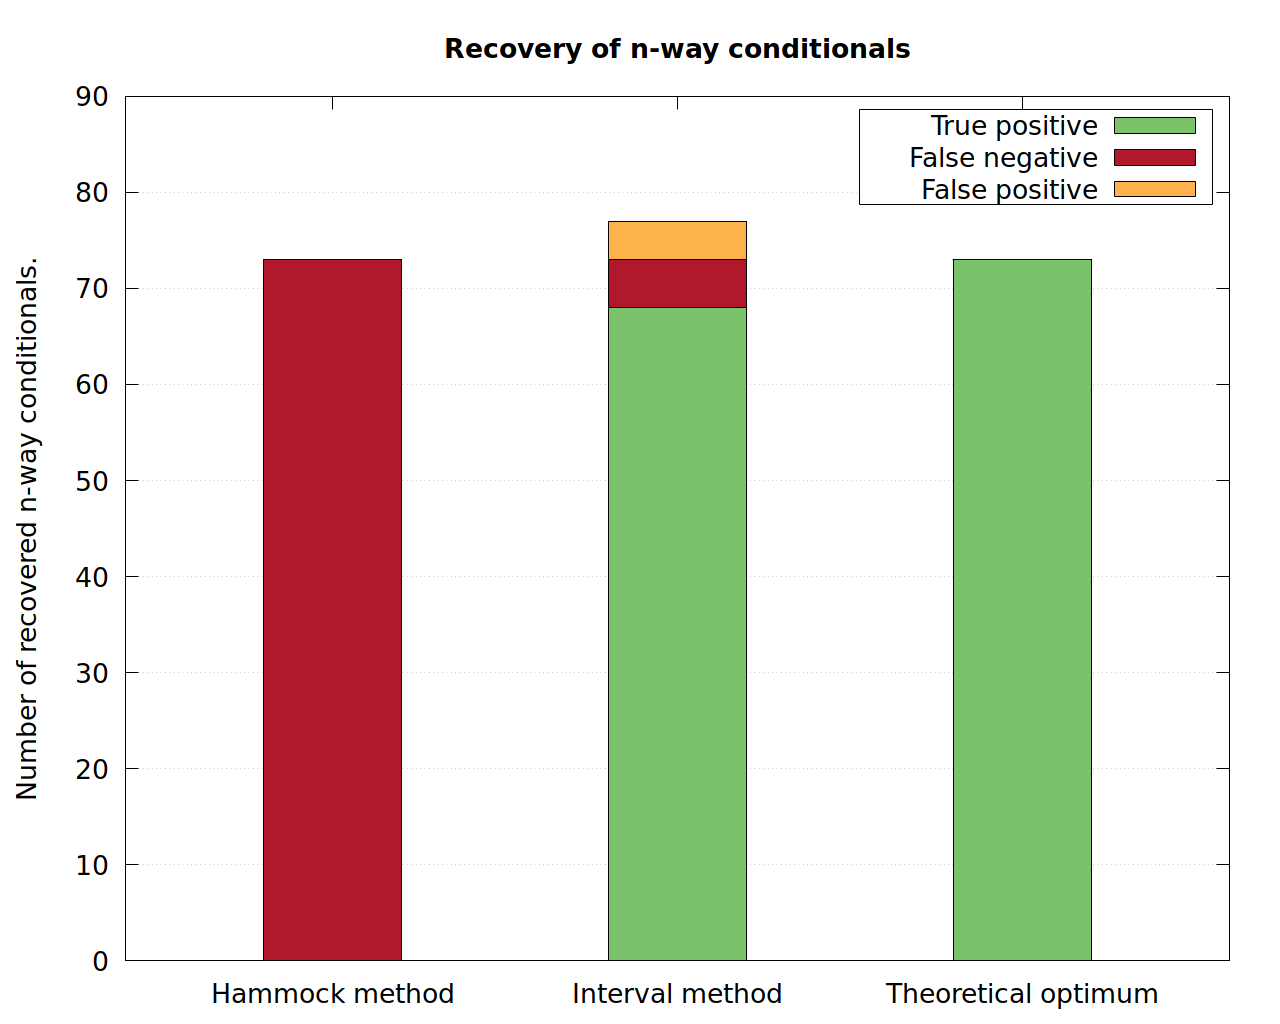
\includegraphics[width=\textwidth]{inc/appendices/test_program_results/sqlite/results_n-way.png}
	\caption{Comparison of control flow recovery results for each method when recovering \textit{n-way conditionals}. The data is based on the test programs of SQLite.}
	\label{fig:sqlite_results_nway}
\end{figure}

\begin{figure}[htbp]
	\centering
	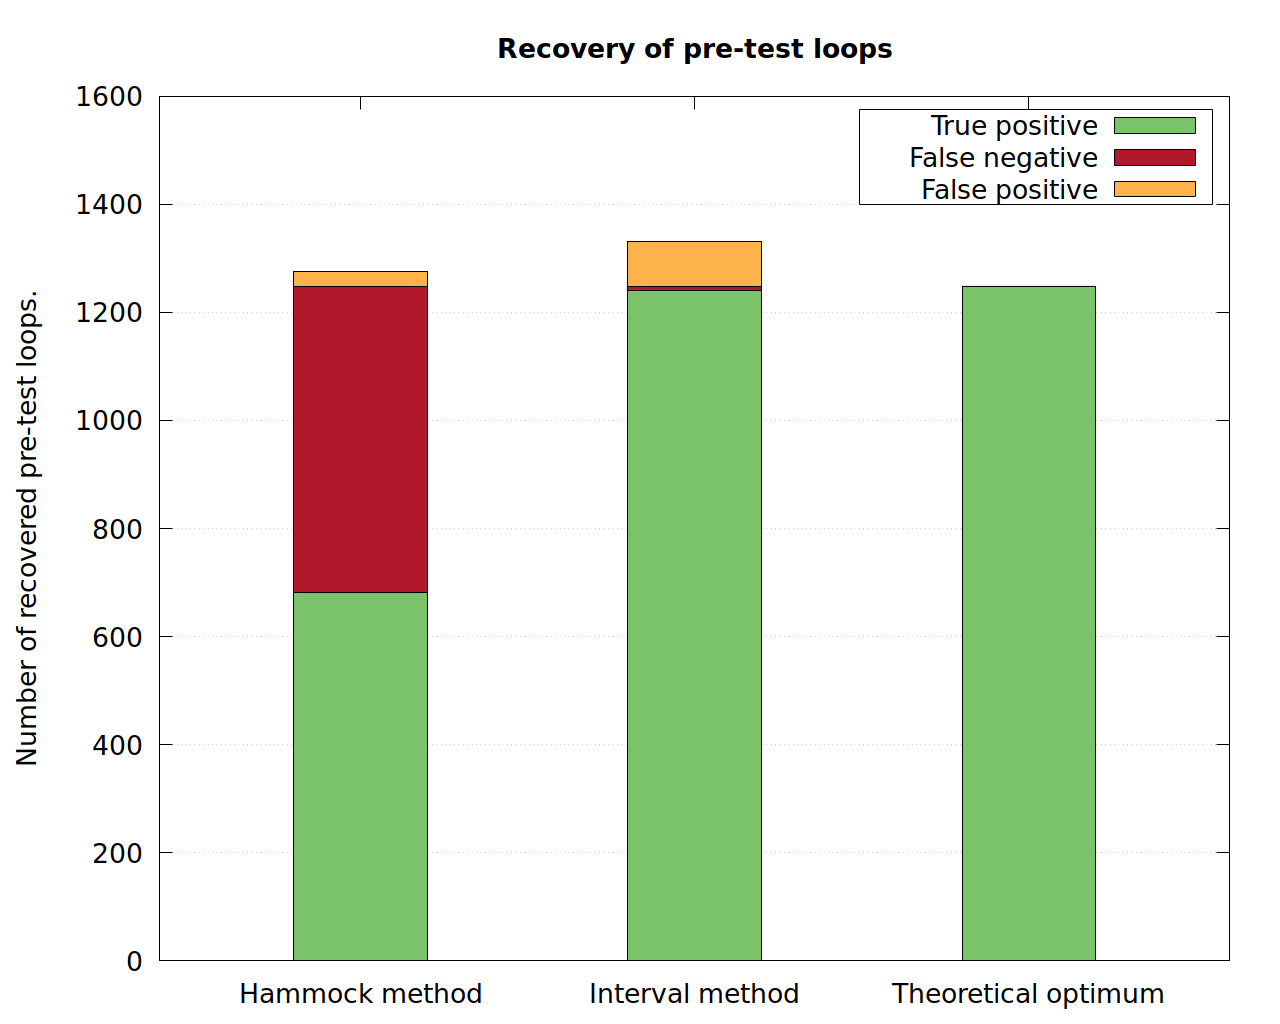
\includegraphics[width=\textwidth]{inc/appendices/test_program_results/sqlite/results_pre_loop.png}
	\caption{Comparison of control flow recovery results for each method when recovering \textit{pre-test loops}. The data is based on the test programs of SQLite.}
	\label{fig:sqlite_results_pre_loop}
\end{figure}

\begin{figure}[htbp]
	\centering
	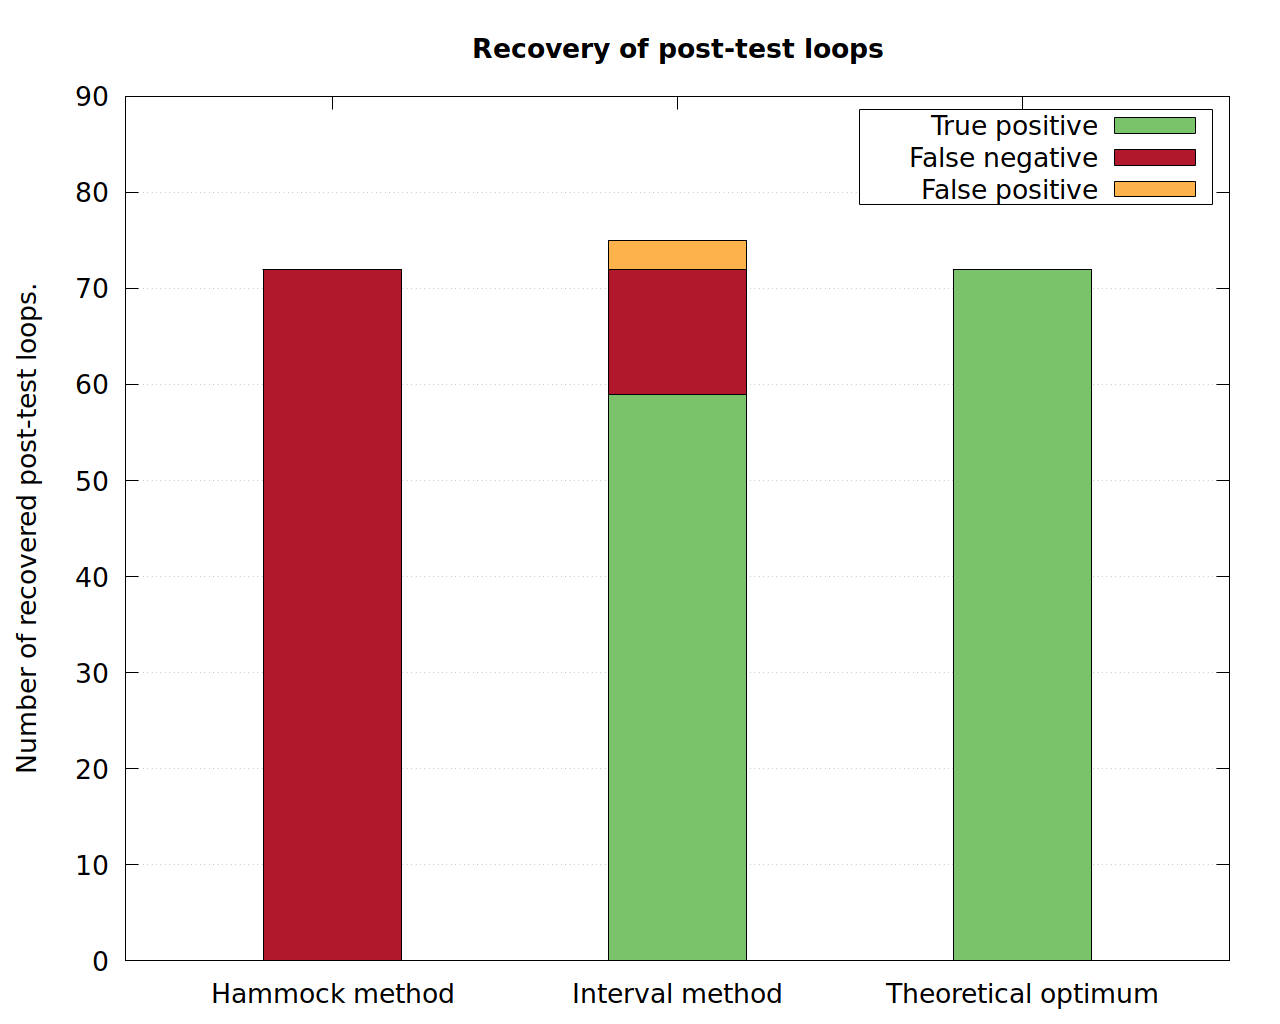
\includegraphics[width=\textwidth]{inc/appendices/test_program_results/sqlite/results_post_loop.png}
	\caption{Comparison of control flow recovery results for each method when recovering \textit{post-test loops}. The data is based on the test programs of SQLite.}
	\label{fig:sqlite_results_post_loop}
\end{figure}
